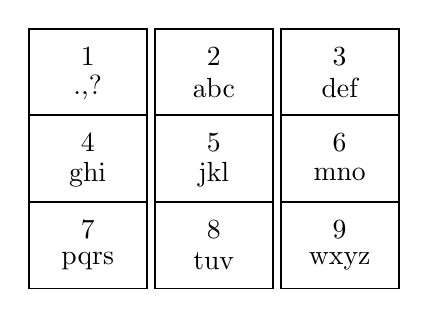
\begin{tikzpicture}[line width=0.7pt]
  % 3x3 keypad grid, each cell 1.6 x 1.1
  \foreach \c [count=\i from 0] in {1,2,3} {
    \draw (\i*1.6,2.2) rectangle (\i*1.6+1.5,3.3);
  }
  \foreach \c [count=\i from 0] in {4,5,6} {
    \draw (\i*1.6,1.1) rectangle (\i*1.6+1.5,2.2);
  }
  \foreach \c [count=\i from 0] in {7,8,9} {
    \draw (\i*1.6,0) rectangle (\i*1.6+1.5,1.1);
  }
  % row 1: numbers and sub-labels
  \node at (0.75,2.95) {1};
  \node at (0.75,2.55) {\text{.,?}};
  \node at (2.35,2.95) {2};
  \node at (2.35,2.55) {abc};
  \node at (3.95,2.95) {3};
  \node at (3.95,2.55) {def};
  % row 2
  \node at (0.75,1.85) {4};
  \node at (0.75,1.45) {ghi};
  \node at (2.35,1.85) {5};
  \node at (2.35,1.45) {jkl};
  \node at (3.95,1.85) {6};
  \node at (3.95,1.45) {mno};
  % row 3
  \node at (0.75,0.75) {7};
  \node at (0.75,0.35) {pqrs};
  \node at (2.35,0.75) {8};
  \node at (2.35,0.35) {tuv};
  \node at (3.95,0.75) {9};
  \node at (3.95,0.35) {wxyz};
\end{tikzpicture}
